\chapter{研究动机与框架概览}
\label{chapter:analysis}

为了帮助研究者更方便的设计和实现神经网络模型,多种流行的神经网络框架被设计出来,并得到了广泛的使用,例如PyTorch, Tensorflow等。
但是目前的框架对于模型并行化训练的支持较为有限,仍然需要研究者手动对模型进行划分,手动管理模型和设备的映射关系。
针对当前框架的不足,我们基于PyTorch设计并实现了\sys{}。
\sys{}提供了对大型神经网络的自动化划分和训练功能,尽可能的简化了大型神经网络的训练流程。
本章节首先介绍大型神经网络训练中的一些难点(\ref{sec:difficulties})和问题分析(\ref{sec:analysis}),然后介绍我们针对大型模型训练所设计的\sys{}框架的整体架构(\ref{sec:design})。

\section{难点与挑战}
\label{sec:difficulties}

超大型神经网络模型由于其含有巨量的参数,因此通常需要将模型划分到多个设备上,使用模型并行化的方式进行分布式训练。
因此,训练超大型模型时,首要难点是如何进行模型划分。
尽管目前PyTorch 1.13 中支持了模型并行化和流水线优化,但是对于模型的划分,仍然依赖于使用者进行手动划分。
另一方面,PyTorch中,对于模型划分的支持只在按层划分的粒度。
\begin{lstlisting}[language=Python, caption={PyTorch 1.13中的流水线并行化}]
 # 分布式训练环境初始化
 os.environ['MASTER_ADDR'] = 'localhost'
 os.environ['MASTER_PORT'] = '29500'
 torch.distributed.rpc.init_rpc('worker', rank=0, world_size=1)
 # 构建流水线
 fc1 = nn.Linear(16, 8).cuda(0)  # 划分到GPU-0
 fc2 = nn.Linear(8, 4).cuda(1)   # 划分到GPU-1
 model = nn.Sequential(fc1, fc2)
 model = Pipe(model, chunks=8)
 input = torch.rand(16, 16).cuda(0)
 output_rref = model(input)
\end{lstlisting}


上述代码展示了来自PyTorch官方文档\footnote[1]{https://pytorch.org/docs/stable/pipeline.html\#torch.distributed.pipeline.sync.Pipe}关于如何将模型划分到多个设备上进行流水线训练的例子。
在这个例子中,首先设置了环境变量,用来指定分布式训练时,需要进行RPC通信的地址。
在6-9行,是模型定义和模型划分,用户需要手动为模型中的每一层分配CUDA设备,在例子中,全连接层fc1被划分到了0号设备,fc2被划分到了1号设备。
在10-12行,被划分好的模型被\texttt{Pipe}包装,进行训练。
\texttt{Pipe}只能接受\texttt{nn.Sequential},也就是模型必须可以表达为连续的若干层,才可以进行进一步的训练。
在原生的PyTorch中,只支持这种对模型进行分层手动划分的方式。
这种方式粒度较粗且缺乏通用性,很难应用到复杂模型上,因为复杂模型难以使用简单的分层结构进行描述。

相比于粗粒度的分层划分,主流的模型划分的工作\upcite{baechi,pesto,rl2,rl1} 针对Tensorflow框架,从模型计算图的角度对模型进行划分。
在Tensorflow 1.x中,用户通过定义计算图来定义模型,计算图可以通过静态分析获得。
而在PyTorch中,用户定义模型和计算图之间仍然具有较大的区别。
PyTorch框架直接对模型的定义代码进行解释执行,在运行时再获取模型的节点(Operator)、节点之间的依赖关系,从而得到运行时动态构建的计算图。
针对PyTorch中大模型的模型并行化训练,我们希望自动化的完成计算图的获取,同时,在对计算图进行划分时,也需要知道每一个节点的内存需求,从而确保划分后,每个设备上分到的节点使用的内存容量不超过设备限制。另外也需要获取每个节点的执行时间,节点与节点之间的通信时间等,来指导模型的划分。在这一过程中,有如下的难点:
% 同时,在对计算图进行划分时,也需要知道每一个节点的内存需求,从而确保划分后,每个设备上分到的节点使用的内存容量不超过设备限制。
% 另外也需要获取每个节点的执行时间,节点与节点之间的通信时间等,来指导模型的划分。
% 1. 用户定义
% 2. 如何获取
% 3. 如何划分模型
\begin{itemize}
	\item \textbf{用户定义模型预处理}:在PyTorch中,用户通常使用高层应用程序接口定义模型。这种高层级的模型在进行训练时,会由训练框架编译为运行时模型。
	用户定义的高层级的模型具有强大的表达能力,方便用户使用简单的代码定义出复杂的模型。
	但是这种高层级的模型往往难以划分。
	因此,需要对用户模型进行一定的预处理,在不改变模型的原有结构和功能的前提下,将模型转化为容易划分的形式。
	% 模型的划分就是计算图的划分,因此我们需要将用户的模型转换为一种计算图的中间表示,划分完成后,再根据划分结果,将中间表示转换回可以进行训练的模型。
	\item \textbf{模型的复杂性}:大型神经网络模型具有复杂的结构,巨大的参数量和很深的网络层次,因此其对应的计算图也有很多节点。每个节点都会进行很多计算,节点需要显存来储存参数,同时节点与节点之间的中间结果也会占用显存,繁多的节点和中间结果让对模型进行分析变得十分困难。
	\item \textbf{硬件环境的复杂性和异构性}:非专有集群中各个设备的型号可能不同,因此它们之间的计算速度和能力也有所不同,在分布式训练中需要控制各个节点之间的计算时间和通信开销,否则会造成任务分配、数据传输等方面的效率问题。
	\item \textbf{模型划分方法的设计}:尽管流水线并行化工作\upcite{gpipe,pipedream,dapple,hippie}被证明可以有效的提高模型并行化中的设备利用率和训练效率,合适的模型划分对于进一步提升训练效率也十分重要。
	通过合理的模型划分,可以有效减少设备之间通信时间,均衡负载,提升训练速度,也可以避免设备出现内存溢出问题。
\end{itemize}


\section{问题分析}
\label{sec:analysis}
% 

针对大型神经网络模型训练中的难点,我们可以将大型神经网络模型的训练问题分解为几个子问题。
\begin{itemize}
	\item \textbf{模型结构理解}:在模型并行化中,需要将模型划分到多个设备上进行训练。这需要让框架对模型的结构有深刻的理解。
	对于现代的深度学习框架来说,通常使用计算图这种中间表示(Intermediate Representation, IR) 来描述运行时的模型。
	我们需要对用户定义的高层级的模型进行分析,从用户的代码中提取出模型的结构信息,并将其转化为计算图这种易于划分的中间表示。我们将这一过程称之为模型结构的理解。
	\item \textbf{模型元信息提取}:在完成“模型结构理解”后,可以得到模型的计算图表示。但是为了下一步的模型划分,还需要对计算图进行分析。框架应该可以自动的提取出会对训练效果产生影响的模型元信息,包括计算图中每个节点的显存需求和计算代价。模型的划分可以简化为寻找计算图中节点到设备的映射,每个设备都会被分配到计算图上的若干节点。因此首先需要保证设备上被分配到的节点使用的显存不会超出设备总显存,从而导致内存溢出问题。
	此外,还需要得知每个节点的前向传播/反向传播用时,节点之间传输的数据量等信息,才能更好的指导模型的划分。
	\item \textbf{训练环境分析}:针对底层硬件设备的异构性,我们需要构建对训练环境进行分析的模块。设备的显存容量制约模型的划分,而设备之间的通信会影响训练的效率,所以我们需要对训练环境进行分析,提取出设备信息,并且对设备之间的通信速度进行分析,减少通信因素对于训练效率的影响。
	\item \textbf{模型划分与训练}:我们需要结合模型结构,模型元信息和具体的训练环境,为模型寻找最优的划分方案,提升训练效率。
	此外,由于划分在计算图层面进行,我们还需要根据对计算图的划分结果,对计算图进行放置,并且对于跨设备的节点,处理它们之间的通信。
	最终完成对划分后的模型的训练。
\end{itemize}

\section{\sys{} 设计}
\label{sec:design}

\begin{figure}[h]
	\centering
	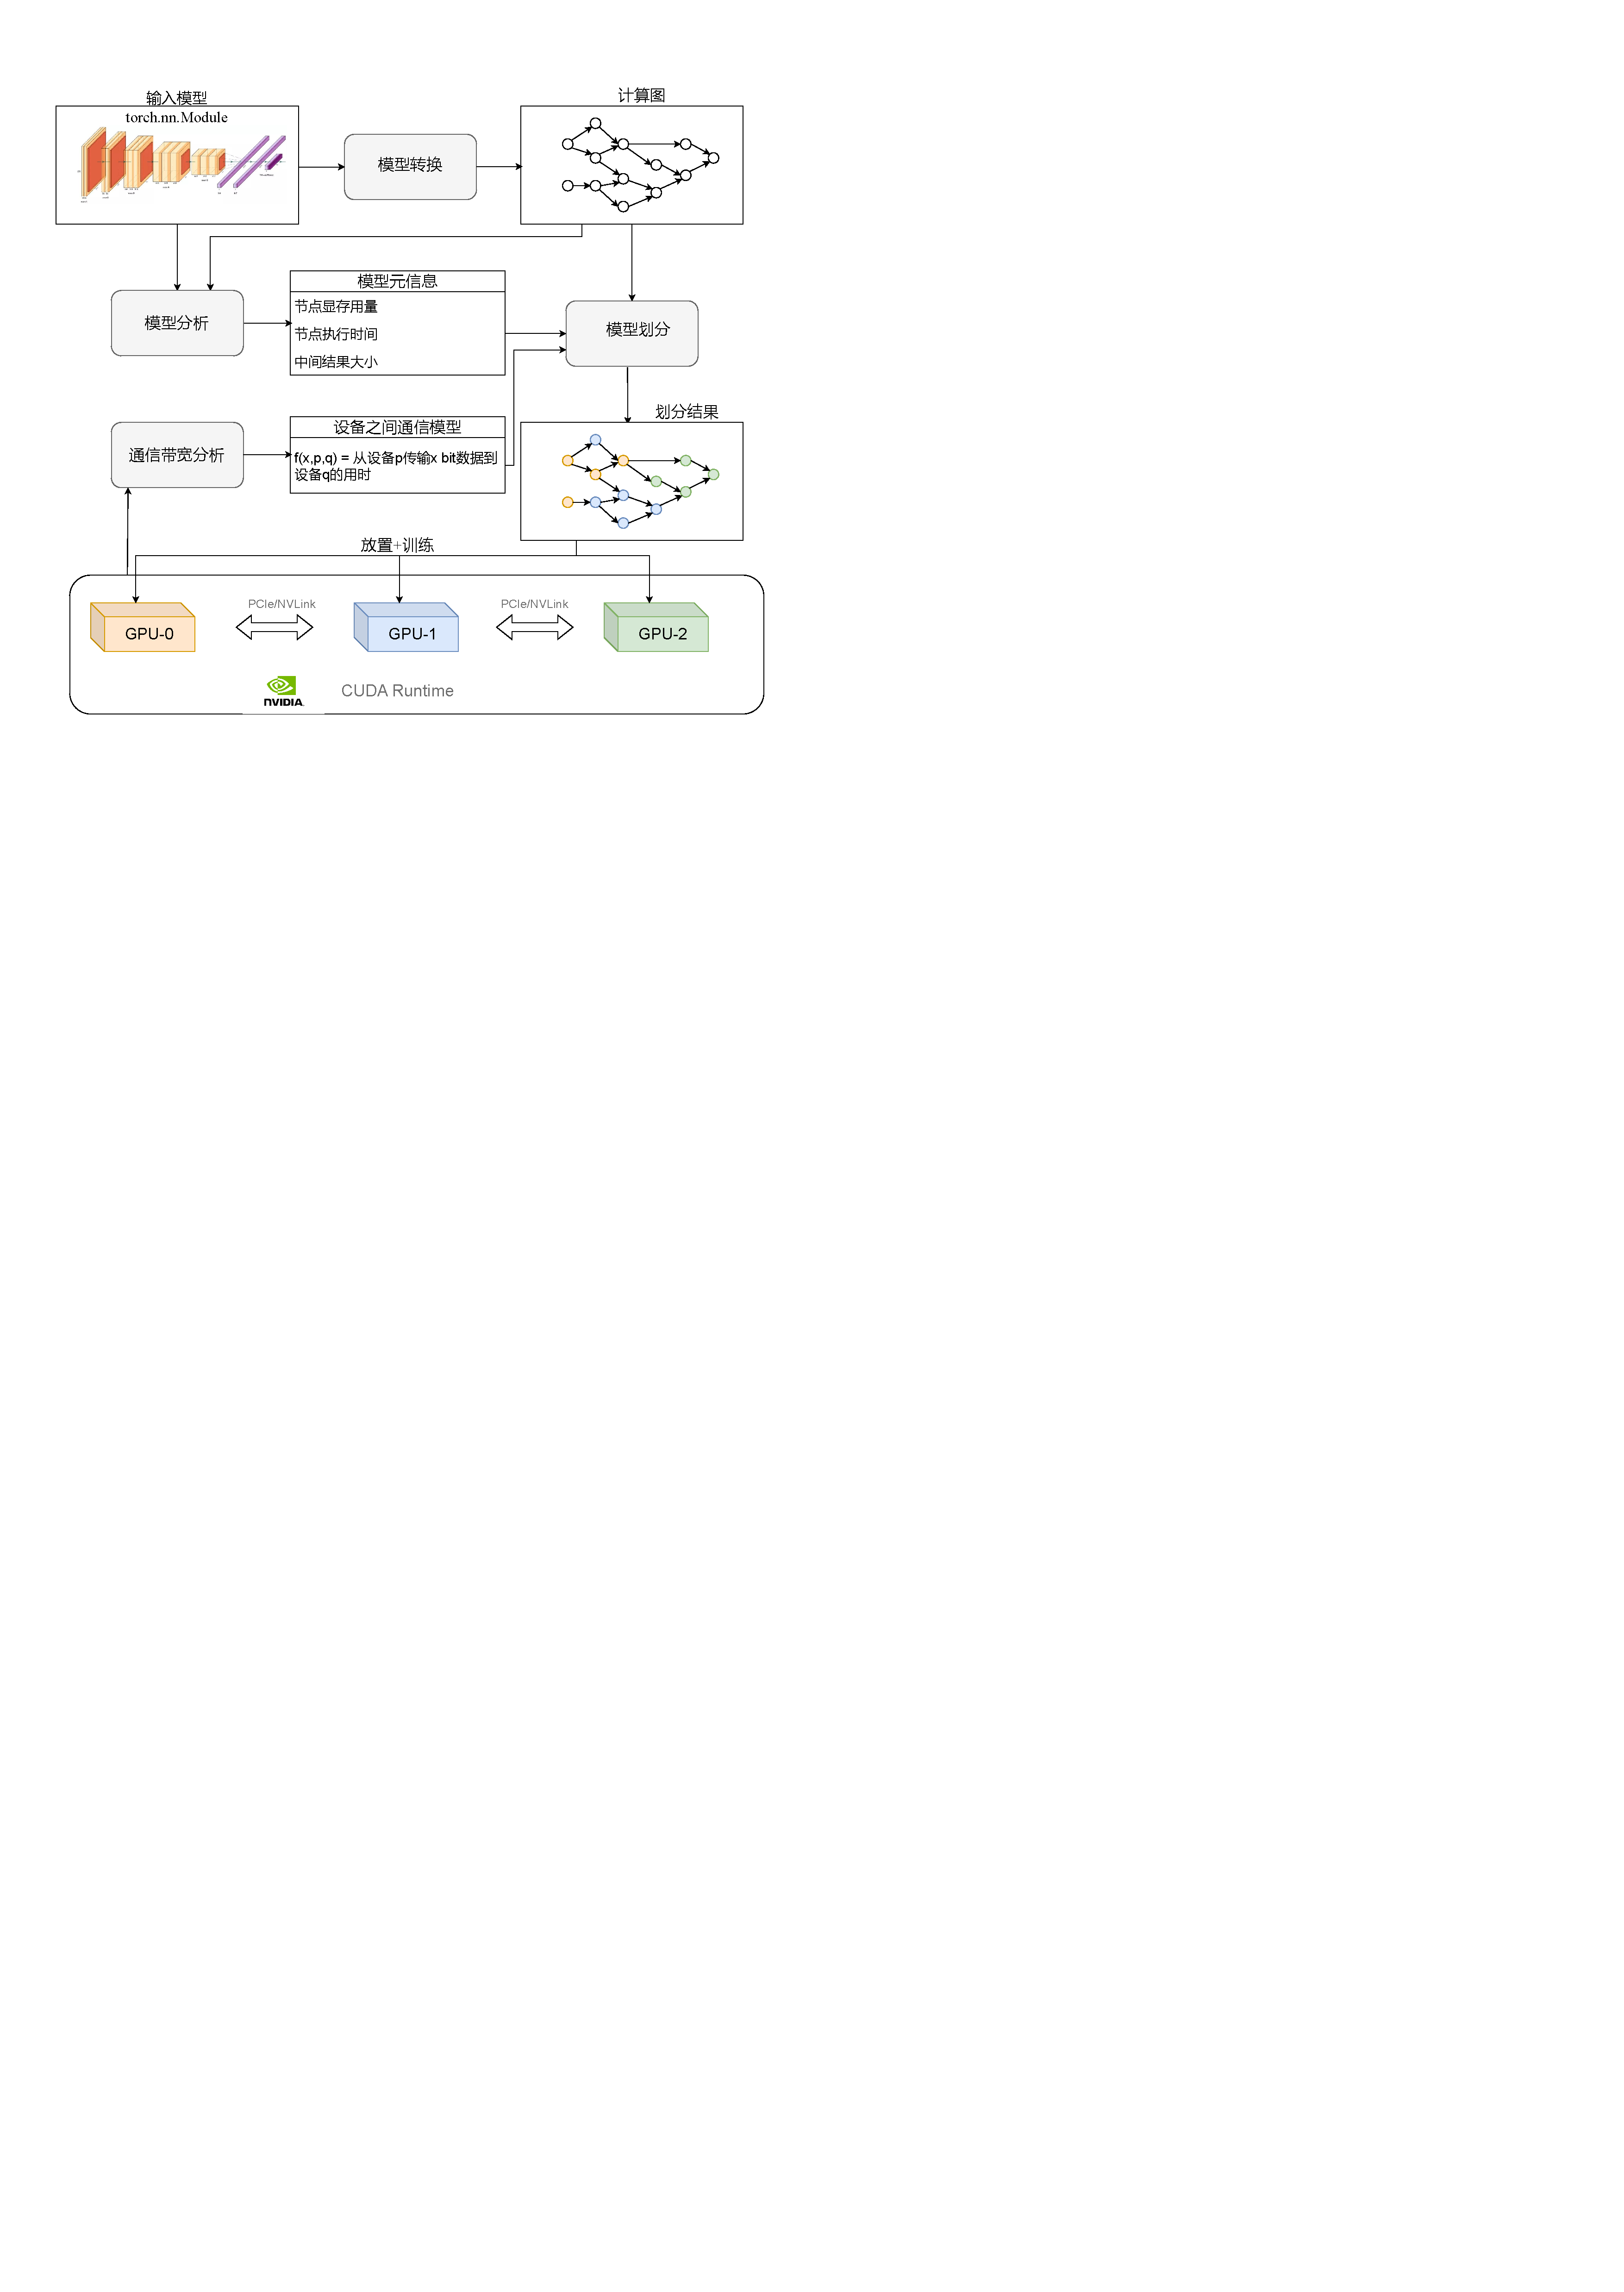
\includegraphics[width=0.95\textwidth]{figure/3-system/arch2.pdf}
	\caption{\sys{} 总体架构}
	\label{fig:arch}
\end{figure}

基于\ref{sec:analysis} 中对大型神经网络模型训练中的问题的分析,我们设计并实现了\sys{}。
\sys{} 是基于PyTorch的,针对大型神经网络进行自动化训练的框架。通过提供自动化的模型分析,硬件环境分析,模型转化,模型划分等功能,尽可能简化大模型等训练流程,减少人工参与,解决大模型难以训练的问题。
\sys{} 支持对通用的PyTorch模型进行训练,无需使用者对模型进行预处理。
\sys{}接受用户定义的模型作为输入,并自动完成模型结构理解,对模型进行转换,得到模型底层计算图的中间表示。然后通过动态分析和静态分析的方式,获得模型的元信息,包括计算图中节点的显存用量,计算图中节点的执行时间等。同时,\sys{} 采集参与训练的硬件的信息,并测试设备之间的点对点通信带宽。
然后模型划分模块接受模型元信息、模型计算图以及设备信息为输入,给出模型的划分结果。最后训练模块根据模型的划分结果进行模型到设备的放置,并启动训练流程,完成训练。
整体框架如图 \ref{fig:arch}所示,各个功能模块的简介如下:
\begin{itemize}
	\item \textbf{模型转换模块}: 负责进行模型结构的理解,实现用户输入的PyTorch模型和计算图中间表示的相互转换,从而允许框架对封装层次较高的模型进行进一步细分。
	\item \textbf{模型分析模块}: 通过动态分析和静态分析的方式,获取模型计算图中每个节点的前向传播/反向传播执行用时,计算图中每条边的传输的数据量,计算图中每个节点使用的内存。
	\item \textbf{通信测试模块}: 对参与训练的设备进行通信带宽的基准测试,来获取设备之间的点对点通信带宽,用于估算跨设备的通信时间。
	\item \textbf{模型划分模块}:模型划分模块是\sys{} 的核心模块,该模块根据模型分析模块和通信测试模块的输出,使用约束优化对模型计算图进行划分。
	\item \textbf{训练运行时模块}:划分好的模型由运行时模块放置到设备上进行训练,改模块根据计算图的划分结果重建模型,并处理节点之间的跨设备通信。
\end{itemize}

\section{本章小结}
本章首先分析了对大型神经网络模型进行训练的难点,例如大型神经网络模型参数量巨大,结构复杂,难以进行分析和预处理,另一方面参与训练的硬件设备也会影响训练的效率。
然后,介绍了对大型神经网络模型进行训练这一问题的分解,我们将问题分解为模型结构理解、模型元信息提取、训练环境分析和模型的划分与训练这四个子问题。
最后,本章介绍了基于PyTorch的\sys{}的设计。
\sys{}提供了对大型神经网络的自动化划分和训练功能,尽可能的简化了大型神经网络的训练流程。

下一章,我们将介绍\sys{}中各个功能模块的实现。